\documentclass[a4paper,10pt]{IEEEtran}
\usepackage{mathptmx}

\usepackage{tabularx} % extra features for tabular environment
\usepackage{amsmath}  % improve math presentation
\usepackage{float}
% \usepackage{pdfpages}

\usepackage{subfig}

\usepackage{graphicx} % takes care of graphics including machinery
\graphicspath{ {./figures_final/} }
%\usepackage[margin=1in,letterpaper]{geometry} % decreases margins
%\usepackage{cite} % takes care of citations
\usepackage[final]{hyperref} % adds hyperlinks inside the generated pdf file
\hypersetup{
    colorlinks=true,       % false: boxed links; true: colored links
    linkcolor=blue,        % color of internal links
    citecolor=blue,        % color of links to bibliography
    filecolor=magenta,     % color of file links
    urlcolor =blue         
}
\usepackage[margin = 1in,headsep=0.5cm,headheight=2cm,letterpaper]{geometry} 

\usepackage{fancyhdr}
\pagestyle{fancy}
\lhead{Student 1 : Ahmet Akman 2442366 \\ Student 2: Kaan Demirkoparan 2442903}
\rhead{Date: \today \\ Group: Friday Morning - 6} 
%\cfoot{center of the footer!}
%\renewcommand{\headrulewidth}{0.1pt}

\title{  EE313 Fall 2022 Project Work  \protect\\ Final Report}
\author{ Ahmet Akman 2442366 -- Kaan Demirkoparan 2442903 }
\date{}
\begin{document}
\thispagestyle{empty}


\maketitle
%\tableofcontents
%\begin{abstract}
%abstract
%\end{abstract}

\section{Introduction}
In this document, the final report of the term project of the EE313 course will be presented. The report is composed of two main parts which describe transmitter and receiver sides. The project specification is to create a telephone pipeline that uses light as a transmission medium.  
\section{General Structure and Design Philisophy}
 The general structure is given in Figure \ref{general}
\begin{figure}[htbp!]
    \centering
    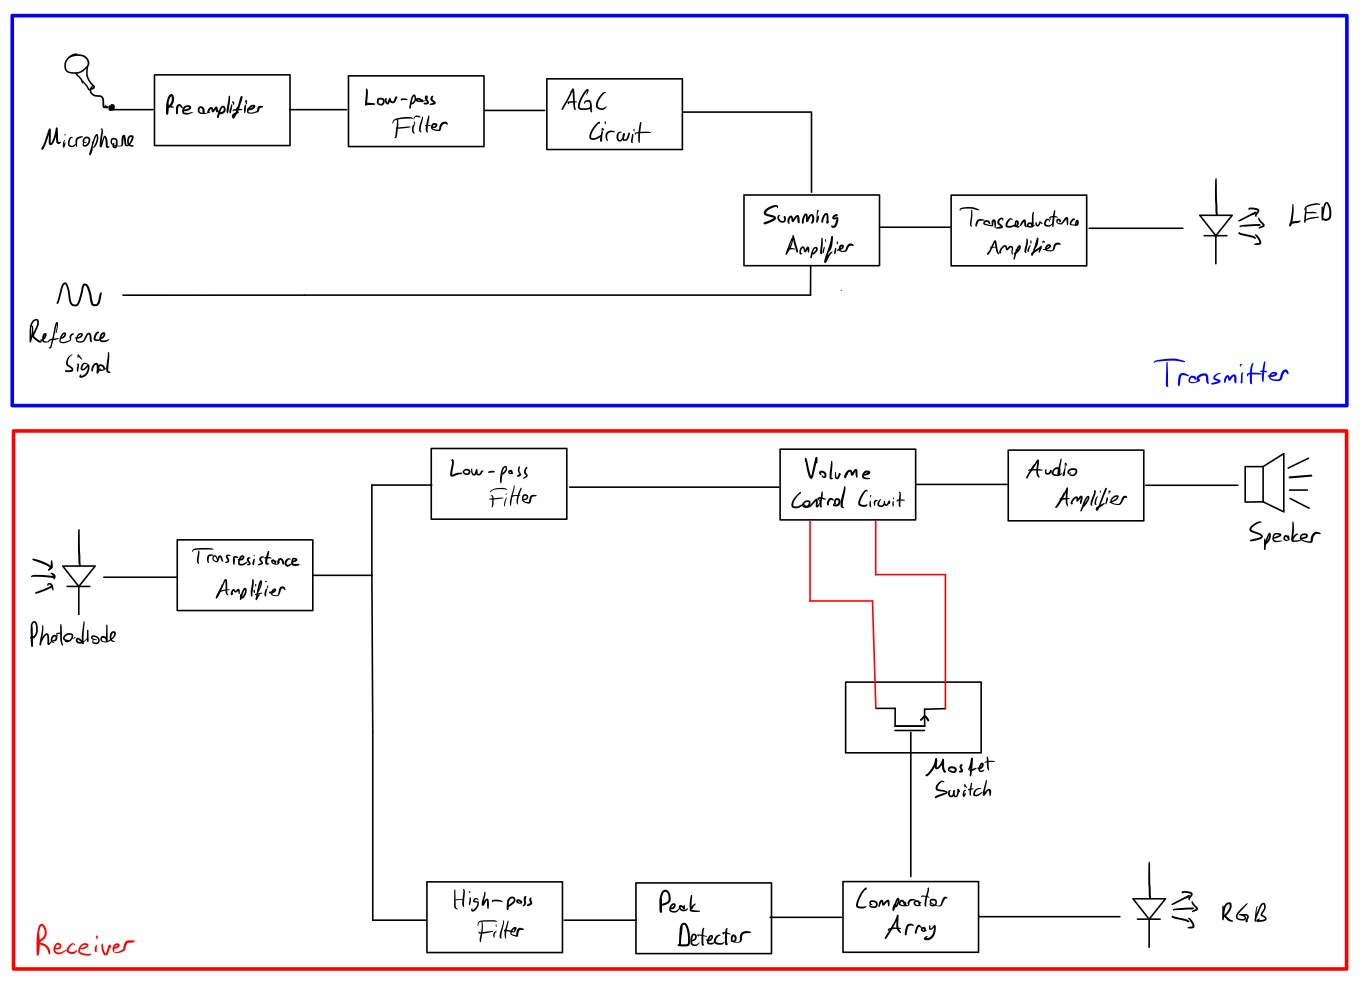
\includegraphics[width = 1\linewidth]{general_structure.jpeg}
    \caption{General Structure}
    \label{general}
\end{figure} 
\section{Transmitter Side}
\subsection{Input and Early Stage Amplification}
The microphone functions as a resistor, with its resistance varying based on the audio waves. To turn audio signals into electrical signals, a voltage divider circuit can be employed. However, the resulting output signal is quite weak, making it susceptible to noise. To mitigate this, the small signal is amplified using a common source or common emitter amplifier, which results in a less noise-sensitive and more usable voltage range signal. Subsequently, this signal is passed through a low pass filter to separate the human voice for further processing.
\subsection{Automatic Gain Control}
\subsection{Reference Signal Summation}

The constant gain audio signal and the high-frequency reference signal should be summed before transmission. This summation process is thought to be applied by adopting a simple opamp summing amplifier.  The schematic is given in \ref{}.
\subsection{Light Transmission}
\section{Receiver Side}
\subsection{Light Receiver}
\subsection{Voice Signal Path}
\subsubsection{Low Pass Filter}
\subsubsection{Speaker Driver}
\subsection{Carrier Signal Path}
\subsubsection{High Pass Filter}
\subsubsection{Signal Level Indication}


\section{Conclusion}

\section*{Appendix}

\end{document}

%%%%%%%%%%%%%%%%%%%%%%   EXAMPLE TABLE   %%%%%%%%%%%%%%%%%%%%%%%%%%%%%%%%
\begin{table}[H]
\begin{center}
    \caption{Resistance reading by color code convention.}
    \vspace{2mm}
    \begin{tabular}{||c | c | c||} 
        \hline
        Color Order & Value & Tolerance \\ [0.5ex] 
        \hline\hline
        Brown / Black / Red / Gold & 1k\( \Omega \) & \( \% \) 5  \\ 
        \hline
        Yellow / Violet / Red / Gold & 4.7k\( \Omega \) & \( \% \) 5   \\
        \hline
        Brown / Grey / Orange / Gold & 18k\( \Omega \) & \( \% \) 5  \\ [1ex] 
        \hline
    \end{tabular}
\end{center}
\end{table}


%%%%%%%%%%%%%%%%%%%%%%   EXAMPLE IMAGE   %%%%%%%%%%%%%%%%%%%%%%%%%%%%%%%%
\begin{figure}[H]
\centering
\includegraphics[width = 0.75\linewidth]{5.png}
\caption{Circuit schematic for the step 5}
\end{figure} 

%%%%%%%%%%%%%%%%%%%%%%   EXAMPLE IMAGE FROM PDF   %%%%%%%%%%%%%%%%%%%%%%%%%%%%%%%%
\begin{figure}[H] \centering{
    \includegraphics[scale=0.25]{2a_plot.pdf}}
    \caption{Experiment 2}
\end{figure}
%%%%%%%%%%%%%%%% Deneme Push